\chapter{Pengujian}

Pada bab ini akan dilakukan pengujian untuk melihat efek penerapan metode \textit{clustering} untuk menyaring fitur lokal terhadap ketepatan dan waktu proses BSIS. Pengujian yang dilakukan ini akan menggunakan cara yang sama dengan yang ada pada \ref{sec:analisis_bsis} tetapi dengan menggunakan \textit{dataset} dan parameter \textit{threshold} yang berbeda. Pada pengujian ini akan digunakan \textit{dataset} GSV (\ref{subsec:dataset_gsv}).

\section{Ide Analisis}
Seperti yang telah dijelaskan sebelumnya, pengujian yang dilakukan pada bagian ini akan mengikuti alur yang telah dilakukan sebelumnya pada \ref{sec:analisis_bsis}. Pengujian ini bertujuan untuk menguji bagaimana penyaringan fitur lokal berdasarkan nilai konsistensi dan keunikannya dapat berpengaruh terhadap hasil saat dilakukan identifikasi terhadap gambar. Pengaruh hasil identifikasi yang diamati merupakan bagaimana tingkat akurasi dan waktu proses yang diperlukan untuk melakukan identifikasi.

Pada pengujian ini penyaringan fitur lokal akan dilakukan menggunakan dua cara. Penyaringan pertama dilakukan dengan menggunakan nilai \textit{threshold} yang didapat dari hasil analisis di \ref{sec:analisis_threshold}. Berdasarkan pada hasil analisis di \ref{sec:analisis_threshold}, penyaringan pertama akan dilakukan dengan menggunakan nilai \textit{threshold} 0.6 untuk konsistensi dan 0.7 untuk keunikan. Penyaringan kedua ditujukan untuk menggunakan nilai \textit{threshold} yang lebih rendah sehingga dapat digunakan sebagai perbandingan. Untuk penyaringan kedua akan ditentukan \textit{threshold} dengan cara yang sama dengan penentuan \textit{threshold} pada analisis di \ref{sec:analisis_threshold}. 

Pengujian ini akan dilakukan menggunakan \textit{dataset} GSV dengan dua ukuran gambar yang berbeda sama seperti pada analisis di \ref{sec:analisis_bsis}. Dua ukuran gambar yang digunakan akan dinamakan GSV 400 dan GSV 600, sesuai ukuran sisi terpanjang pada gambar-gambar yang digunakan. Berbeda dengan analisis pada \ref{sec:analisis_bsis}, pada pengujian ini ukuran dari gambar di data \textit{test} akan disesuaikan dengan ukuran gambar yang digunakan pada \textit{dataset}. Pengujian juga akan dilakukan dengan menggunakan dua metode ekstraksi fitur lokal yaitu SIFT dan ORB.

\section{Penentuan Threshold dan Hasil Analisis}
\subsection{Metode SIFT}
\subsubsection{GSV 400}
Sebaran nilai konsistensi dan keunikan untuk \textit{dataset} GSV 400 dapat dilihat pada Gambar~\ref{fig:consistency_gsv400_pengujian_sift} dan Gambar~\ref{fig:uniqueness_gsv400_pengujian_sift}.
\begin{figure}[H]
	\centering
	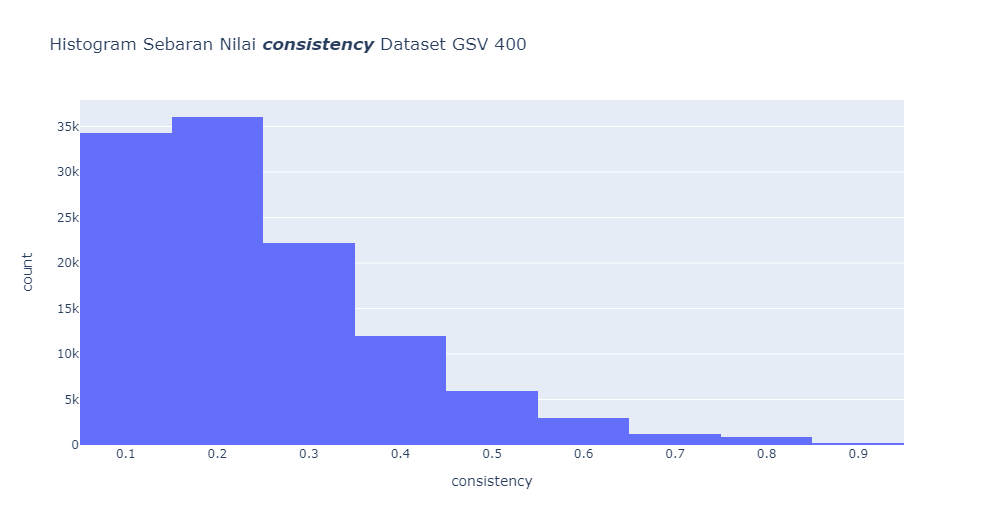
\includegraphics[width=\textwidth]{consistency_gsv400.png}
	\caption{Histogram sebaran nilai keunikan pada \textit{Dataset} GSV 400.}
	\label{fig:consistency_gsv400_pengujian_sift}
\end{figure}

\begin{figure}[H]
	\centering
	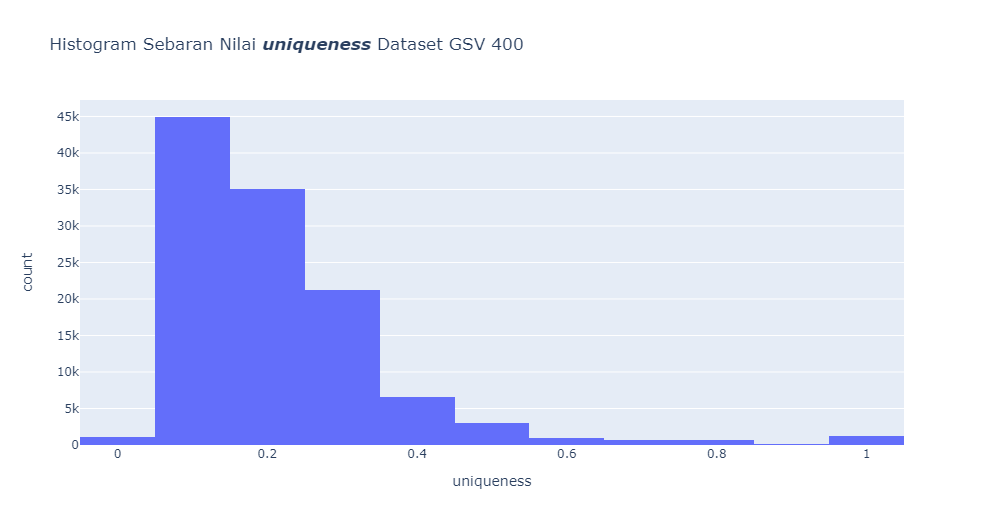
\includegraphics[width=\textwidth]{uniqueness_gsv400.png}
	\caption{Histogram sebaran nilai keunikan \textit{Dataset} GSV 400.}
	\label{fig:uniqueness_gsv400_pengujian_sift}
\end{figure}
Dengan melihat sebaran nilai konsistensi dan keunikan pada Gambar~\ref{fig:consistency_gsv400_pengujian_sift} dan Gambar~\ref{fig:uniqueness_gsv400_pengujian_sift} maka akan digunakan nilai \textit{threshold} senilai 0.3 untuk konsistensi dan 0.3 untuk keunikan. Kedua nilai tersebut didapat dengan cara yang sama dengan yang dilakukan pada \ref{sec:analisis_bsis}. 

Pengujian pada \textit{dataset} GSV 400 akan dilakukan dengan menggunakan 3 set \textit{threshold} yang berbeda. Ketiga set \textit{threshold} yang digunakan adalah sebagai berikut:
\begin{itemize}
	\item Keseluruhan
	\begin{itemize}
		\item konsistensi: 0.0
		\item keunikan: 0.0
	\end{itemize}
	\item Threshold 1
	\begin{itemize}
		\item konsistensi: 0.3
		\item keunikan: 0.3
	\end{itemize}
	\item Threshold 2
	\begin{itemize}
		\item konsistensi: 0.6
		\item keunikan: 0.7
	\end{itemize}
\end{itemize}
Telah dilakukan pengujian terhadap data \textit{test} dengan menggunakan ketiga set nilai \textit{threshold} tersebut. Hasil dari pengujian dapat dilihat pada Tabel~\ref{tab:pengujian_sift_gsv400}
\begin{table}[H]
	\centering
	\begin{tabular}{|l|l|l|l|}
		\hline
		& \textbf{Total Waktu Ekstrak (s)} & \textbf{Total Waktu BSIS(s)} & \textbf{Akurasi (\%)} \\ \hline
		Keseluruhan & 1.25	&	90.99                    & 94                    \\ \hline
		Threshold 1 & 1.29	&	24.30                    & 84                    \\ \hline
		Threshold 2 & 1.21	&	13.67                    & 10                    \\ \hline
	\end{tabular}
	\caption{Hasil pengujian pada \textit{dataset} GSV 400.}
	\label{tab:pengujian_sift_gsv400}
\end{table}

\subsubsection{GSV 600}
Sebaran nilai konsistensi dan keunikan untuk \textit{dataset} GSV 600 dapat dilihat pada Gambar~\ref{fig:consistency_gsv600_pengujian_sift} dan Gambar~\ref{fig:uniqueness_gsv600_pengujian_sift}.
\begin{figure}[H]
	\centering
	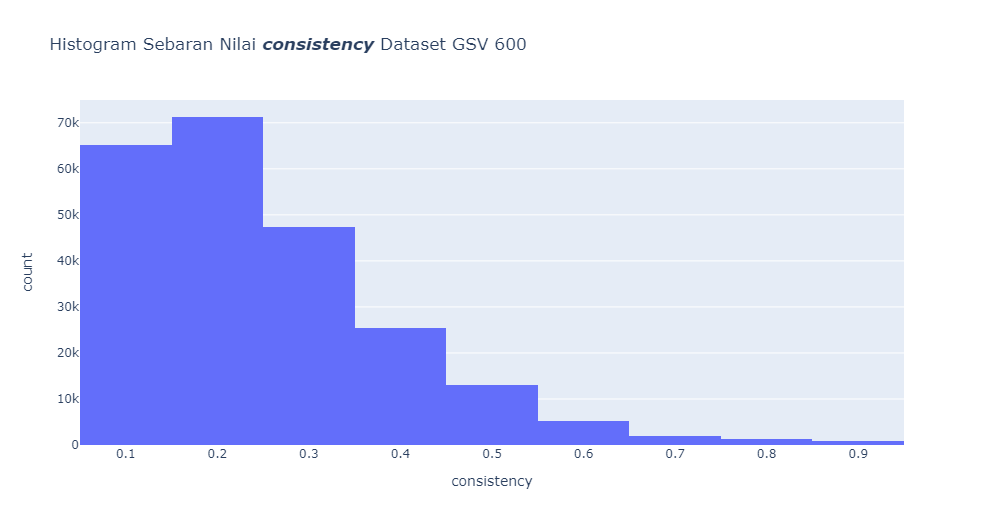
\includegraphics[width=\textwidth]{consistency_gsv600.png}
	\caption{Histogram sebaran nilai keunikan pada \textit{Dataset} GSV 600.}
	\label{fig:consistency_gsv600_pengujian_sift}
\end{figure}

\begin{figure}[H]
	\centering
	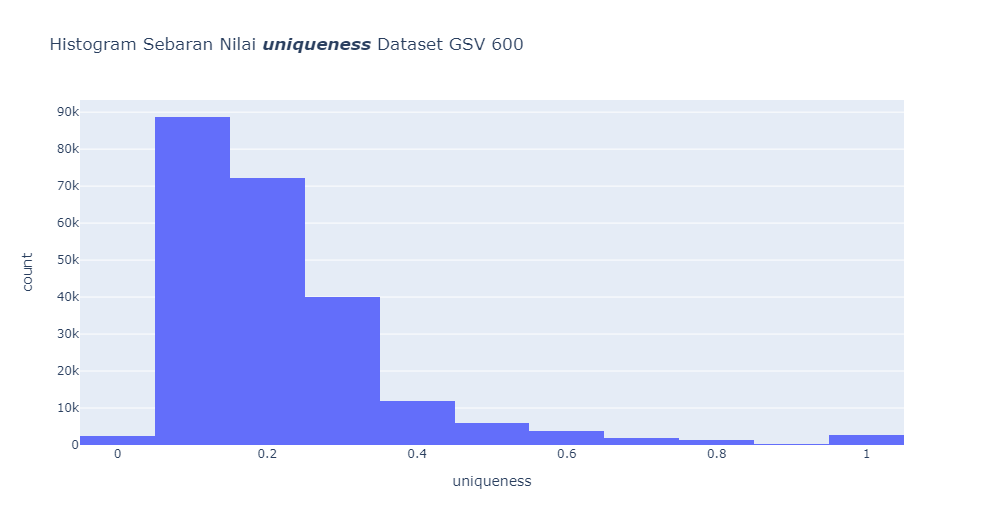
\includegraphics[width=\textwidth]{uniqueness_gsv600.png}
	\caption{Histogram sebaran nilai keunikan \textit{Dataset} GSV 600.}
	\label{fig:uniqueness_gsv600_pengujian_sift}
\end{figure}
Dengan menggunakan cara yang sama seperti sebelumnya, berdasarkan sebaran yang dapat dilihat pada Gambar~\ref{fig:consistency_gsv600_pengujian_sift} dan Gambar~\ref{fig:uniqueness_gsv600_pengujian_sift} maka akan digunakan nilai \textit{threshold} senilai 0.3 untuk konsistensi dan 0.3 untuk keunikan. Tiga set \textit{threshold} yang digunakan pada pengujian \textit{dataset} ini adalah sebagai berikut:
\begin{itemize}
	\item Keseluruhan
	\begin{itemize}
		\item konsistensi: 0.0
		\item keunikan: 0.0
	\end{itemize}
	\item Threshold 1
	\begin{itemize}
		\item konsistensi: 0.3
		\item keunikan: 0.3
	\end{itemize}
	\item Threshold 2
	\begin{itemize}
		\item konsistensi: 0.6
		\item keunikan: 0.7
	\end{itemize}
\end{itemize}
Setelah dilakukan pengujian terhadap \textit{dataset} GSV 600 dengan menggunakan tiga set \textit{threshold} tersebut didapat hasil yang dapat dilihat pada Tabel~\ref{tab:pengujian_sift_gsv600}.

\begin{table}[H]
	\centering
	\begin{tabular}{|l|l|l|l|}
		\hline
		& \textbf{Total Waktu Ekstrak (s)} & \textbf{Total Waktu BSIS(s)} & \textbf{Akurasi (\%)} \\ \hline
		Keseluruhan & 2.69 & 187.64                   & 100                    \\ \hline
		Threshold 1 & 2.57 & 47.58                    & 84                    \\ \hline
		Threshold 2 & 2.75 & 20.55                    & 16                    \\ \hline
	\end{tabular}
	\caption{Hasil pengujian pada \textit{dataset} GSV 600.}
	\label{tab:pengujian_sift_gsv600}
\end{table}

Hasil pada Tabel~\ref{tab:pengujian_sift_gsv400} dan Tabel~\ref{tab:pengujian_sift_gsv600} menunjukkan nilai \textit{threshold} yang didapat dari hasil analisis pada \textit{threshold} (\ref{sec:analisis_threshold}) memberikan hasil BSIS dengan akurasi yang sangat rendah. Cara penentuan \textit{threshold} dengan melihat hasil pada gambar tersebut ternyata tidak efektif jika digunakan untuk melakukan identifikasi. Hal ini mungkin dikarenakan dalam melakukan identifikasi gambar banyak fitur lokal yang berasal bukan dari bagian yang merupakan logo atau objek penting, tetapi sebenarnya berguna dalam identifikasi.

\subsection{Metode ORB}
Pada pengujian dengan metode ORB ini hanya akan digunakan satu set \textit{threshold}. \textit{Threshold} yang digunakan adalah \textit{threshold} yang didapat dari melihat hasil sebaran nilai konsistensi dan keunikan. Nilai \texttt{threshold} yang didapat dengan melihat hasilnya pada gambar seperti pada \ref{sec:analisis_threshold} tidak digunakan pada pengujian ini, karena pada penelitian ini tidak dilakukan analisis \textit{threshold} dengan menggunakan metode ORB. 

\subsubsection{GSV 400}
Sebaran nilai konsistensi dan keunikan untuk \textit{dataset} GSV 400 dapat dilihat pada Gambar~\ref{fig:consistency_gsv400_pengujian_orb} dan Gambar~\ref{fig:uniqueness_gsv400_pengujian_orb}.
\begin{figure}[H]
	\centering
	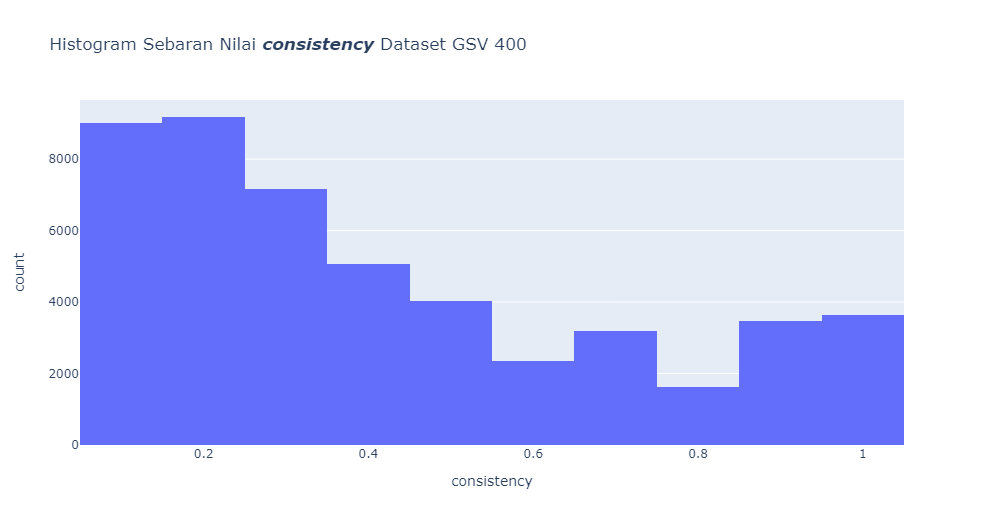
\includegraphics[width=\textwidth]{consistency_gsv400_orb.png}
	\caption{Histogram sebaran nilai keunikan pada \textit{Dataset} GSV 400.}
	\label{fig:consistency_gsv400_pengujian_orb}
\end{figure}

\begin{figure}[H]
	\centering
	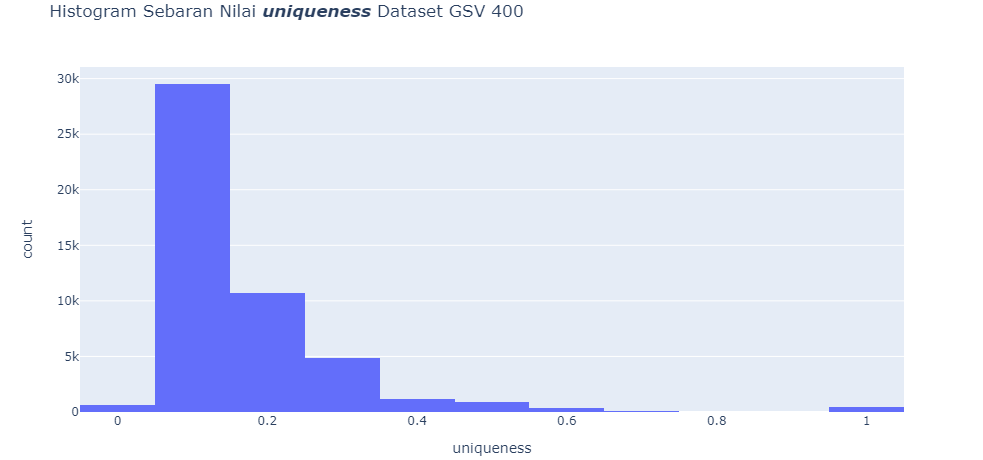
\includegraphics[width=\textwidth]{uniqueness_gsv400_orb.png}
	\caption{Histogram sebaran nilai keunikan \textit{Dataset} GSV 400.}
	\label{fig:uniqueness_gsv400_pengujian_orb}
\end{figure}
Dari kedua histogram pada Gambar~\ref{fig:consistency_gsv400_pengujian_orb} dan Gambar~\ref{fig:uniqueness_gsv400_pengujian_orb} ditetapkan nilai \textit{threshold} untuk konsistensi senilai 0.3 dan untuk keunikan senilai 0.3. Dua set \textit{threshold} yang digunakan pada pengujian ini adalah sebagai berikut:
\begin{itemize}
	\item Keseluruhan
	\begin{itemize}
		\item konsistensi: 0.0
		\item keunikan: 0.0
	\end{itemize}
	\item Threshold 1
	\begin{itemize}
		\item konsistensi: 0.3
		\item keunikan: 0.3
	\end{itemize}
\end{itemize}
Setelah dilakukan pengujian terhadap \textit{dataset} didapat hasil seperti yang dapat dilihat pada Tabel~\ref{tab:pengujian_orb_gsv400}
\begin{table}[H]
	\centering
	\begin{tabular}{|l|l|l|l|}
		\hline
		& \textbf{Total Waktu Ekstrak (s)} & \textbf{Total Waktu BSIS(s)} & \textbf{Akurasi (\%)} \\ \hline
		Keseluruhan & 0.17 & 51.12                   & 76                    \\ \hline
		Threshold 1 & 0.33 & 1.81                    & 28                    \\ \hline
	\end{tabular}
	\caption{Hasil pengujian pada \textit{dataset} GSV 400.}
	\label{tab:pengujian_orb_gsv400}
\end{table}
\subsubsection{GSV 600}
Sebaran nilai konsistensi dan keunikan untuk \textit{dataset} GSV 600 dapat dilihat pada Gambar~\ref{fig:consistency_gsv600_pengujian_orb} dan Gambar~\ref{fig:uniqueness_gsv600_pengujian_orb}.
\begin{figure}[H]
	\centering
	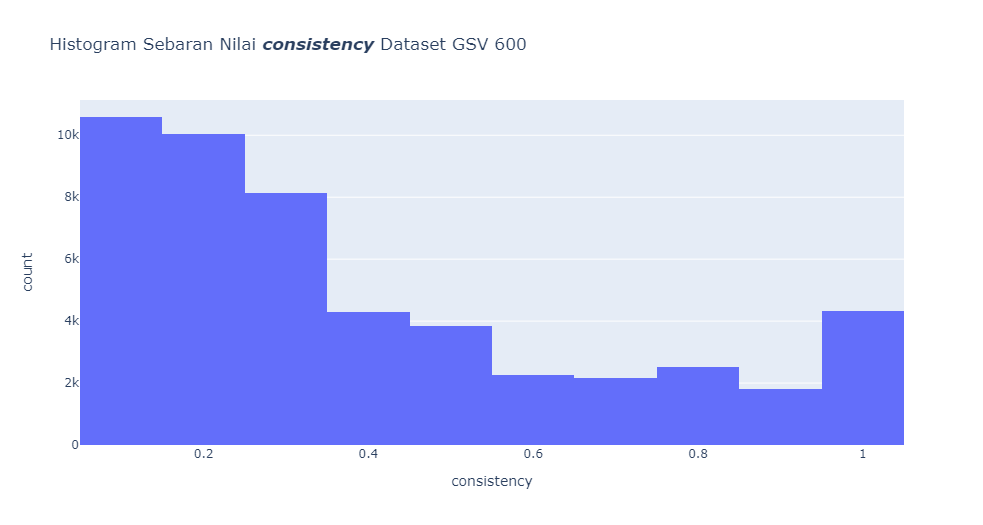
\includegraphics[width=\textwidth]{consistency_gsv600_orb.png}
	\caption{Histogram sebaran nilai keunikan pada \textit{Dataset} GSV 600.}
	\label{fig:consistency_gsv600_pengujian_orb}
\end{figure}

\begin{figure}[H]
	\centering
	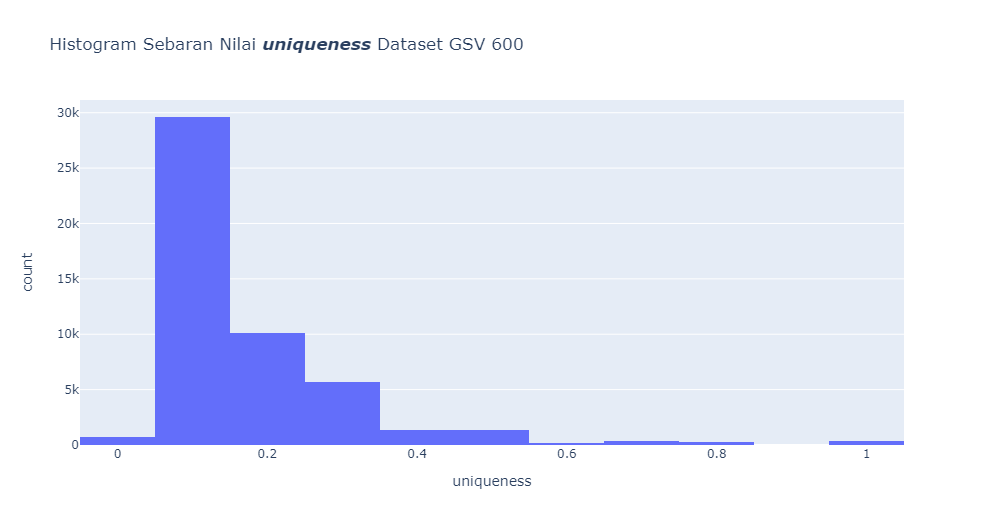
\includegraphics[width=\textwidth]{uniqueness_gsv600_orb.png}
	\caption{Histogram sebaran nilai keunikan \textit{Dataset} GSV 600.}
	\label{fig:uniqueness_gsv600_pengujian_orb}
\end{figure}
Dapat dilihat dari kedua histogram di Gambar~\ref{fig:consistency_gsv600_pengujian_orb} dan Gambar~\ref{fig:uniqueness_gsv600_pengujian_orb} bahwa sebaran nilai konsistensi dan keunikan untuk GSV 600 sama dengan sebaran pada GSV 400. Dari sebaran nilai yang sama antara GSV 400 dan GSV 600 ini maka untuk GSV 600 dapat digunakan set \textit{threshold} yang sama dengan GSV 400. Dua set \textit{threshold} yang digunakan pada pengujian GSV 600 ini adalah sebagai berikut:
\begin{itemize}
	\item Keseluruhan
	\begin{itemize}
		\item konsistensi: 0.0
		\item keunikan: 0.0
	\end{itemize}
	\item Threshold 1
	\begin{itemize}
		\item konsistensi: 0.3
		\item keunikan: 0.3
	\end{itemize}
\end{itemize}
Setelah dilakukan pengujian terhadap \textit{dataset} didapat hasil seperti yang dapat dilihat pada Tabel~\ref{tab:pengujian_orb_gsv600}
\begin{table}[H]
	\centering
	\begin{tabular}{|l|l|l|l|}
		\hline
		& \textbf{Total Waktu Ekstrak (s)} & \textbf{Total Waktu BSIS(s)} & \textbf{Akurasi (\%)} \\ \hline
		Keseluruhan & 0.31 & 51.10                   & 78                    \\ \hline
		Threshold 1 & 0.29 & 2.99                    & 20                    \\ \hline
	\end{tabular}
	\caption{Hasil pengujian pada \textit{dataset} GSV 600.}
	\label{tab:pengujian_orb_gsv600}
\end{table}

\section{Analisis Hasil Pengujian}
Pada bagian analisis ini akan dibandingkan hasil dari pengujian antara SIFT dan ORB yang telah dilakukan. Pengujian yang dilakukan dengan menggunakan \textit{threshold} dari hasil analisis \textit{threshold} tidak akan ikut dibandingkan, karena nilai \textit{threshold} tersebut hanya digunakan pada pengujian dengan SIFT. Perbandingan yang dilakukan akan dibagi berdasarkan ukuran gambar yang digunakan. Hasilnya dapat dilihat pada subbab-subbab berikut ini.

\subsection{GSV 400}
\begin{table}[H]
	\centering
	\begin{tabular}{|l|l|l|l|l|}
		\hline
		&             & \textbf{Total Waktu Ekstrak (s)} & \textbf{Total Waktu BSIS (s)} & \textbf{Akurasi (\%)} \\ \hline
		\multicolumn{1}{|c|}{\multirow{2}{*}{SIFT}} & Keseluruhan & 1.25                             & 90.99                         & 94                    \\ \cline{2-5} 
		\multicolumn{1}{|c|}{}                      & Threshold 1 & 1.29                             & 24.30                         & 84                    \\ \hline
		\multirow{2}{*}{ORB}                        & Keseluruhan & 0.17                             & 51.12                         & 76                    \\ \cline{2-5} 
		& Threshold 1 & 0.33                             & 1.81                          & 28                    \\ \hline
	\end{tabular}
	\caption{Hasil perbandingan pengujian SIFT dan ORB pada \textit{dataset} GSV 400.}
	\label{tab:perbandingan_gsv400}
\end{table}
Dari hasil pada Tabel~\ref{tab:perbandingan_gsv400} terlihat bahwa pada terdapat perbedaan hasil yang cukup signifikan antara SIFT dan ORB. Terlihat bahwa dari SIFT dan ORB terdapat penurunan waktu ekstraksi fitur yang cukup signifikan. Total waktu BSIS pada ORB juga menurun secara signifikan dibandingkan dengan SIFT, tetapi penurunan ini lebih dikarenakan jumlah fitur lokal yang dihasilkan ORB tidak sebanyak yang dihasilkan oleh SIFT. Nilai akurasi dari SIFT dan ORB juga mengalami penurunan yang signifikan. Akurasi dari ORB ada pada angka yang termasuk rendah terutama pada hasil yang telah disaring, hasil ini berbeda dari hasil yang didapat dari pengujian pada analisis di \ref{sec:analisis_orb}. Pada pengujian di analisis sebelumnya identifikasi dengan menggunakan metode ORB masih menghasilkan nilai akurasi yang cukup tinggi walaupun nilainya masih lebih kecil dari SIFT.

\subsection{GSV 600}
\begin{table}[H]
	\centering
	\begin{tabular}{|l|l|l|l|l|}
		\hline
		&             & \textbf{Total Waktu Ekstrak (s)} & \textbf{Total Waktu BSIS (s)} & \textbf{Akurasi (\%)} \\ \hline
		\multicolumn{1}{|c|}{\multirow{2}{*}{SIFT}} & Keseluruhan & 2.69                             & 187.64                        & 100                   \\ \cline{2-5} 
		\multicolumn{1}{|c|}{}                      & Threshold 1 & 2.57                             & 47.58                         & 84                    \\ \hline
		\multirow{2}{*}{ORB}                        & Keseluruhan & 0.31                             & 51.10                         & 78                    \\ \cline{2-5} 
		& Threshold 1 & 0.29                             & 2.99                          & 20                    \\ \hline
	\end{tabular}
	\caption{Hasil perbandingan pengujian SIFT dan ORB pada \textit{dataset} GSV 600.}
	\label{tab:perbandingan_gsv600}
\end{table}
Hasil yang dapat dilihat pada Tabel~\ref{tab:perbandingan_gsv600} menunjukkan pola yang sama dari SIFT dan ORB, di mana SIFT memerlukan waktu yang lebih lama baik dari waktu ekstrak maupun waktu untuk BSIS, tetapi juga menghasilkan akurasi yang lebih tinggi. Pada \textit{dataset} ini waktu yang diperlukan baik untuk ekstrak maupun BSIS lebih tinggi dari waktu yang diperlukan \textit{dataset} GSV 400. Waktu yang lebih lama tersebut dikarenakan ukuran gambar yang lebih besar sehingga lebih banyak fitur lokal yang dapat dihasilkan dari tahap ekstraksi.

%\section{Hasil}
%\begin{table}[H]
%	\centering 
%	\begin{tabular}{|cl|llll|}
%		\hline
%		\multicolumn{2}{|c|}{\multirow{2}{*}{Dataset}}               & \multicolumn{4}{c|}{\begin{tabular}[c]{@{}c@{}}Threshold\\ (konsistensi;keunikan)\end{tabular}}                           \\ \cline{3-6} 
%		\multicolumn{2}{|c|}{}                                       & \multicolumn{1}{c|}{0.0;0.0} & \multicolumn{1}{c|}{0.2;0.2} & \multicolumn{1}{c|}{0.4;0.4} & \multicolumn{1}{c|}{0.7;0.8} \\ \hline
%		\multicolumn{1}{|c|}{\multirow{2}{*}{400}} & Total Waktu (s) & \multicolumn{1}{l|}{90.99}   & \multicolumn{1}{l|}{45.12}   & \multicolumn{1}{l|}{17.71}   & 13.67                        \\ \cline{2-6} 
%		\multicolumn{1}{|c|}{}                     & Akurasi (\%)    & \multicolumn{1}{l|}{94}      & \multicolumn{1}{l|}{92}      & \multicolumn{1}{l|}{40}      & 20                           \\ \hline
%		\multicolumn{1}{|c|}{\multirow{2}{*}{600}} & Total Waktu (s) & \multicolumn{1}{l|}{187.64}  & \multicolumn{1}{l|}{95.77}   & \multicolumn{1}{l|}{34.40}   & 20.55                        \\ \cline{2-6} 
%		\multicolumn{1}{|c|}{}                     & Akurasi (\%)    & \multicolumn{1}{l|}{100}     & \multicolumn{1}{l|}{92}      & \multicolumn{1}{l|}{58}      & 32                           \\ \hline
%	\end{tabular}
%\end{table}

